%%%%%%%%%%%%%%%%%%%%%%%%%%%%%%%%%%%%%%%%%
% a0poster Portrait Poster
% LaTeX Template
% Version 1.0 (22/06/13)
%
% The a0poster class was created by:
% Gerlinde Kettl and Matthias Weiser (tex@kettl.de)
% 
% This template has been downloaded from:
% http://www.LaTeXTemplates.com
%
% License:
% CC BY-NC-SA 3.0 (http://creativecommons.org/licenses/by-nc-sa/3.0/)
%
%%%%%%%%%%%%%%%%%%%%%%%%%%%%%%%%%%%%%%%%%

%----------------------------------------------------------------------------------------
%	PACKAGES AND OTHER DOCUMENT CONFIGURATIONS
%----------------------------------------------------------------------------------------

\documentclass[a0,portrait]{a0poster}

\usepackage{multicol} % This is so we can have multiple columns of text side-by-side
\columnsep=80pt % This is the amount of white space between the columns in the poster
\columnseprule=3pt % This is the thickness of the black line between the columns in the poster

\usepackage[svgnames]{xcolor} % Specify colors by their 'svgnames', for a full list of all colors available see here: http://www.latextemplates.com/svgnames-colors

%\usepackage{times} % Use the times font
%\usepackage{palatino} % Uncomment to use the Palatino font

\usepackage{graphicx} % Required for including images
\graphicspath{{figures/}} % Location of the graphics files
\usepackage{booktabs} % Top and bottom rules for table
\usepackage[font=small,labelfont=bf]{caption} % Required for specifying captions to tables and figures
\usepackage{amsfonts, amsmath, amsthm, amssymb} % For math fonts, symbols and environments
\usepackage{wrapfig} % Allows wrapping text around tables and figures
\usepackage{natbib}
\usepackage{hyperref}
\usepackage{wrapfig}

\begin{document}

%----------------------------------------------------------------------------------------
%	POSTER HEADER 
%----------------------------------------------------------------------------------------

% The header is divided into two boxes:
% The first is 75% wide and houses the title, subtitle, names, university/organization and contact information
% The second is 25% wide and houses a logo for your university/organization or a photo of you
% The widths of these boxes can be easily edited to accommodate your content as you see fit

\begin{minipage}[b]{0.70\linewidth}
\veryHuge \color{NavyBlue} \textbf{Gender and linguistic variation:} \color{Black}\\ % Title
\Huge\textit{a role for hormonal organising effects}\\[2cm] % Subtitle
\huge \textbf{Anne-marie Karatzenis, Josef Fruehwald, Danielle Turton \\\& Joel C. Wallenberg}\\[0.5cm] % Author(s)
\huge Newcastle University and University of Edinburgh \\[0.4cm] % University/organization
\Large \texttt{joel.wallenberg@ncl.ac.uk}\\
\end{minipage}
%
\begin{minipage}[b]{0.25\linewidth}

\includegraphics[width=11cm]{ncltitle2.jpg}
\includegraphics[width=11cm]{edin.jpg}\\
\end{minipage}

\vspace{1cm} % A bit of extra whitespace between the header and poster content

%----------------------------------------------------------------------------------------

\begin{multicols}{2} % This is how many columns your poster will be broken into, a portrait poster is generally split into 2 columns

%----------------------------------------------------------------------------------------
%	ABSTRACT
%----------------------------------------------------------------------------------------

\color{Navy} % Navy color for the abstract

\begin{abstract}

Below we describe a small, completed pilot study, a larger pilot study in progress, and a future large-scale investigation into whether there is an endocrine basis for differential production of linguistic variants by gender. While results are preliminary, our initial pilot shows that prenatal testosterone, as measured by the 2D/4D digit ratio, is likely to affect the frequencies of linguistic variants a person produces in naturalistic, running speech.

\end{abstract}

%----------------------------------------------------------------------------------------
%	INTRODUCTION
%----------------------------------------------------------------------------------------

\color{SaddleBrown} % SaddleBrown color for the introduction

\section*{Introduction}


\textbf{Gender:} part of a person's internal sense of self, usually related to social roles, and probably related to brain structures.\\
\textbf{Sex:} a rough description of a person's physical primary and secondary sexual characteristics, generally excluding the brain (in reference to humans).

\begin{itemize}
		\item \textbf{Linguistic sex/gender effects:} it is well known that speaker-sex has a stochastic effect on the frequency with which linguistic variants are used, with women leading changes from below.
		\item \textbf{Hormonal Organising Effects:} the action of sex steroids, during the critical period for sexual differentiation 
		(\textsl{in utero}, esp. weeks 8-24 for humans), affecting primary/secondary sex characteristics, and gender:
			\begin{itemize}
				\item Behaviour: mating behaviours in mammals, sexuality and gender identity in humans, pair-bonding and other behaviours in birds.
				\item Brain morphology: e.g. the sexually-dimorphic nucleus of the pre-optic area in mammals, including humans, with a correlate in birds; also e.g. parts of the avian song system \citep[][]{balthazartetal2009}.
				\item Not to be confused with hormone activational, or circulating, effects, which are often independent.
			\end{itemize}
	\end{itemize}


%----------------------------------------------------------------------------------------
%	OBJECTIVES
%----------------------------------------------------------------------------------------

\color{DarkSlateGray} % DarkSlateGray color for the rest of the content

\section*{Research Questions}


\begin{enumerate}
\item Is gender, understood as a non-binary continuum, a better predictor for the frequencies of linguistic variants than sex?
\item Is there a sociobiological explanation for the reported sex effect in change from below (contra, e.g. \citealt{labov2001, eckert2011}) ?
	\begin{itemize}
		\item And is it, in reality, a continuous gender effect rather than sex?
	\end{itemize}
\item Can we add to existing evidence that there is a continuous biological basis for the continuum of gender identity?
	\begin{itemize}
	\item Is linguistic production more closely correlated with both biological gender and a nuanced notion of gender identity than other behaviours (e.g. sexuality)?
	\end{itemize}


\end{enumerate}

\section*{Background}
\subsection*{A biological basis for gender}



\begin{itemize}
	\item \citet{hinesetal2004}: Congenital Adrenal Hyperplasia (CAH) in XX, AFAB individuals has a significant effect on both sexuality and less female-typical/identifying gender identity both in childhood and adulthood, compared to controls.
	\item \citet{berenbaumbailey2003}: CAH and parents' identification of ``tomboy'' were significant predictors of gender identity in XX, AFAB individuals aged 18 and younger. (Interestingly, genitial appearance was not, even when partly masculinized.)
	\item \citet{hinesetal2002}: In a non-clinical population (Avon Longitudinal Study of Parents and Children, ALSPAC \citealt{alspac2001}), found significant effect of maternal testosterone on childhood gender-role behaviour in XX, AFAB individuals aged 3.5, as assessed by the Pre-School Activities Index.
	\item \citet{auyeungetal2009} confirmed \citet{hinesetal2002}'s results predicting PSAI with amniotic fluid samples, gestation weeks 11-21, sample of 112 male, 100 female.
	\item Many other human and animal studied have found relationships between perinatal T and gendered behaviour or sexuality \citep[see][for reviews]{hines2006, balthazart2011}.
\end{itemize}

\subsection*{The Filled Pause Change in Progress}

%\begin{multicols}{2}
\begin{minipage}[b]{0.6\linewidth}
\begin{center}\vspace{1cm}
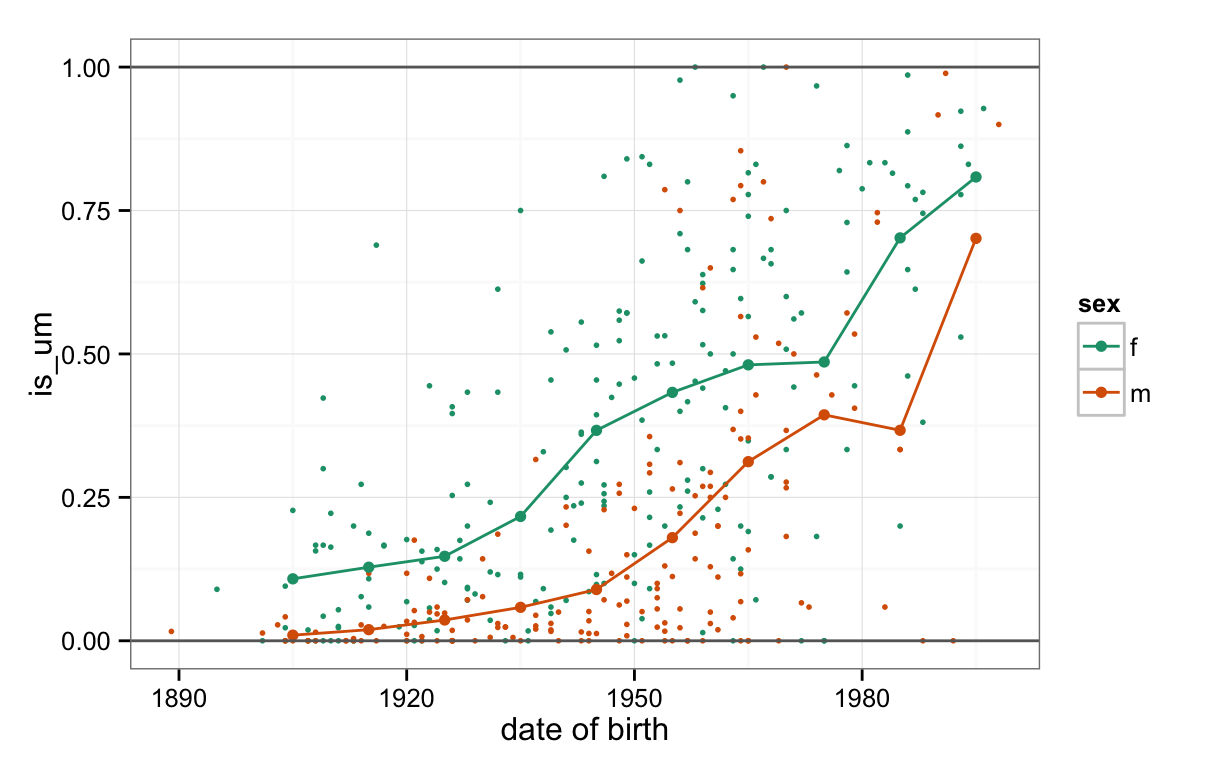
\includegraphics[width=.85\linewidth]{um.png}
\end{center}
\end{minipage}
\begin{minipage}[b]{0.3\linewidth}
\begin{center}
\captionof{figure}{\color{Green} Replacement of \textsl{uh} by \textsl{um} in the Philadelphia Neighborhood Corpus \citep{labovrosenfelder2011}, N = 308 speakers}
\end{center}
\end{minipage}
%\end{multicols}

\subsection*{A Proxy for Perinatal T: 2D/4D ratio}


%INSERT PICTURE FROM BALTHAZART, OR OF MY OWN HANDS
%\begin{wrapfigure}{l}{0.3\linewidth}
%  \begin{center}
%  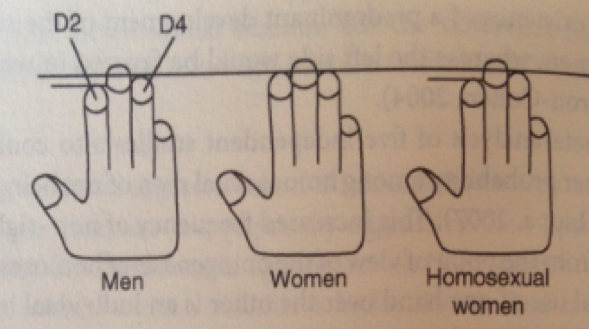
\includegraphics[width=0.3\linewidth]{balthazart108hands.png}
%  \end{center}
%  \caption{Birds}
%\end{wrapfigure}



%\begin{minipage}[.5\textheight]{\textwidth}

\begin{multicols}{2}

\begin{itemize}
	\item Broadly speaking, female ratios closer to 1, on average around 0.973, and male ratios smaller, average: 0.955 \citep[][107]{balthazart2011}.
	
	\item Sexual orientation: see extensive references in \citet{balthazart2011}, as well as rat models.
	\item 2D/4D difference in ``butch'' vs. ``femme'' self-report (gender?) in self-identified lesbians, with ``femme'' non-distinct from straight controls, but ``butch'' more masculinized \citep{brownetal2002}
	\item Experimentally manipulated in Wistar rats: maternal testosterone manipulation and direct pre-natal manipulation results in lower 2D/4D ratios in female rats, and also behavioral similarities to male rats in open field motor activity\citep{talarovicovaetal2009}.
\end{itemize}
%\end{minipage}

%\begin{minipage}[0.2\textheight]{0.2\textwidth}
\begin{center}
  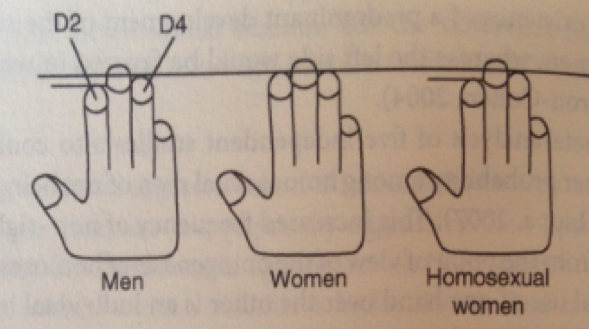
\includegraphics[width=0.5\linewidth]{balthazart108hands.png}
  \end{center}
\end{multicols}
%\end{minipage}

%----------------------------------------------------------------------------------------
%	MATERIALS AND METHODS
%----------------------------------------------------------------------------------------

\section*{Pilot Study}

%\subsection*{Hypothesis}

In a population of assigned-female-at-birth and female-identifying participants, controlled for age, location, and SEC, the 2D/4D ratio will be a strong predictor of the frequency of filled pause variants in naturalistic speech.

%------------------------------------------------
\subsection*{Methods}
\begin{itemize}
	\item N = 10 women (AFAB and female-identified), aged 18 to 22.
	\item All participants native speakers from the Tyneside dialect area (all within 20 miles of Newcastle, most closer).
	\item Standard sociolinguistic interviews, controlled for topics, recorded with either a, H1 or H4 Zoom.
	\item 2D/4D measurements made either physically on hands and with tracings (for 1st cohort), or with digital Vernier calipers from photocopies (2nd cohort). (Photocopies were found to be the second most reliable measurement technique for 2D/4D by \citealt{allawayetal2009})
	%BASAL CREASE? KNUCKLE?
\end{itemize}


%----------------------------------------------------------------------------------------
%	RESULTS 
%----------------------------------------------------------------------------------------

\section*{Results}



%ADD IN RESULTS FROM THE EMAIL FROM JOE HERE 
The 2D/4D digit ratio is nearly \textbf{as good a predictor in our all-female sample} for the frequency of \textsl{um/uh} pause fillers  \textbf{as male vs. female sex} is in large spoken corpora.
\begin{center}
\noindent\textbf{Interpretation: less pre-natal testosterone $\rightarrow$ more \textsl{um}.}
\end{center}
\begin{wraptable}{l}{13.9cm} % Left or right alignment is specified in the first bracket, the width of the table is in the second
\begin{tabular}{l c}
\toprule
\textbf{Sample} & \textbf{Effect Size}\\
\midrule
Sex, HCRC Maptask & 2.3\\
Sex, Fischer Corpus & 1.37\\
Sex, PNC & 1.31\\
\textbf{Finger Ratio, our Pilot 1} & \textbf{1.17}\\
Sex, Switchboard Corpus & 1.03\\
Sex, British National Corpus & 0.45\\
\bottomrule
\end{tabular}
\captionof{table}{\color{Green} This effect size against the female effect size in other Spoken English corpora (source for latter: Wieling et al \textsl{forthcoming})}
\end{wraptable}

To scale the ratio so that larger ratios don't unduly affect the model, we used the measure $log_1.2(ratio)$. Thus, the effect size is difference between a 1:1 ratio to a 1.2:1 ratio (the largest ratio in the data).

Finger ratio effect size, and 95\% CI based on 1000 bootstrap replicates (CI excludes 0): 1.17 (0.34, 2.17):

A mixed effects logistic model containing the finger ratio has a smaller AIC, and a significant likelihood ratio test.

Probably due to the small sample size, a permutation test (randomly permuting subjects' finger ratios) isn't significant, p = 0.163, and model excluding ratio has a smaller BIC.


\begin{center}\vspace{1cm}

\includegraphics[width=0.8\linewidth]{placeholder}
\captionof{figure}{\color{Green} Figure caption}
\end{center}\vspace{1cm}


\section*{Future Research}

\begin{multicols}{2}
\subsection*{Pilot Study 2}
\begin{itemize}
\item More Tyneside speakers.
\item Self-report as ``tomboy''
\item Scan 2D/4D and use digital calipers with GNU Image Modification Package \citep[][]{allawayetal2009}.
\item A better, continuous self-report task for gender identity:
\end{itemize}

\begin{center}
  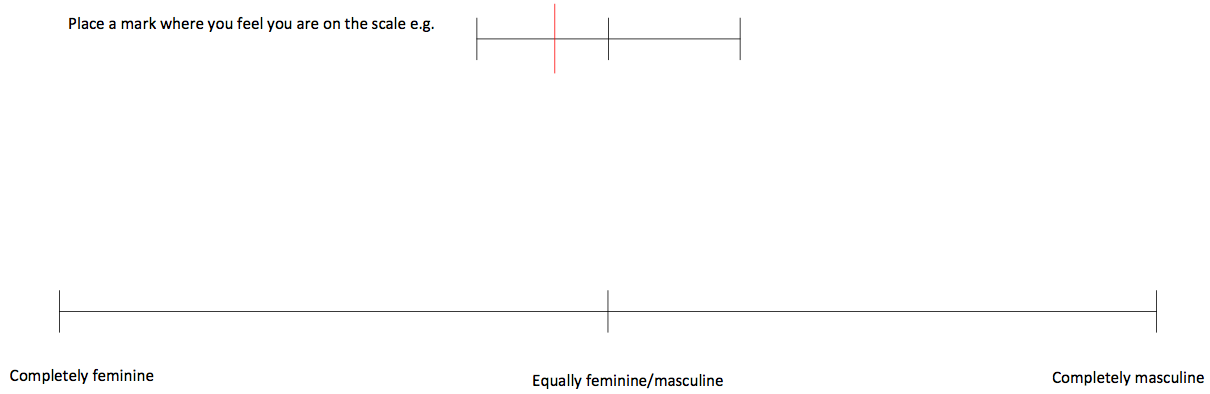
\includegraphics[width=1\linewidth]{scale.png}
  \end{center}
  
\end{multicols}
\subsection*{Large-scale study}

%ALSPAC, etc. - mostly take from Joel's York talk

\begin{itemize}
	\item As above, esp. regarding continuous gender report, but...
	\item 200 participants from ALSPAC, with poor assays for maternal T and estradiol. 
	\item Standard sociolinguistic interview procedures, with semi-automatic extraction of changes in progress from FAVE-aligned transcriptions:
	\begin{itemize}
		\item Categorical change from below: \textsl{um/uh}
		\item Some below-consciousness phonetic and phonological variables (maybe production and perception), e.g. /uw/-fronting, pre aspiration, ...
	\end{itemize}
	\begin{center}
\begin{itemize}
\item If linguistic variables are learnt differentially depending on how masculinised brain structures have been by pre-natal androgen levels, then:
\end{itemize}
\end{center} 
\begin{itemize}
	\item Within a given sex cohort (i.e. genital-sex, or sex designated at birth), more advanced linguistic variants correspond to lower levels of pre-natal T, and perhaps other androgens (esp. women).
	\item If the gender effect in language is purely social, then we should see no effect of hormones within each sex (only between sexes).
\end{itemize}
\end{itemize}

%----------------------------------------------------------------------------------------
%	CONCLUSIONS
%----------------------------------------------------------------------------------------

\color{SaddleBrown} % SaddleBrown color for the conclusions to make them stand out

\section*{Conclusions}

\begin{itemize}
\item 
\end{itemize}

\color{DarkSlateGray} % Set the color back to DarkSlateGray for the rest of the content


 %----------------------------------------------------------------------------------------
%	REFERENCES
%----------------------------------------------------------------------------------------
\end{multicols}
%\nocite{*} % Print all references regardless of whether they were cited in the poster or not
\bibliographystyle{linquiry2} % Plain referencing style
\bibliography{posterrefs} % Use the example bibliography file sample.bib

%----------------------------------------------------------------------------------------
%	ACKNOWLEDGEMENTS
%----------------------------------------------------------------------------------------

\section*{Acknowledgements}

Most thanks to our two RAs, Claire Cochrane and Caitlin Halfacre. Thanks also go particularly to Jacques Balthazart and Daniel Nettle, for extensive discussion of the issues and methodologies, and to Charles Yang for discussion regarding social networks. A number of individuals in the Newcastle transgender community have graciously given their input into how we ask for gender self-reports. Thank you also to audiences at Newcastle University's Centre for Behaviour and Evolution and the University of York's Language and Evolution Workshop.

%----------------------------------------------------------------------------------------


\end{document}